\documentclass[12pt,a4paper]{article}

\usepackage[utf8]{inputenc}
\usepackage[T1]{fontenc}
\usepackage{setspace}
\usepackage{geometry}
\usepackage{microtype}
\usepackage{ragged2e}
\usepackage{indentfirst}
\usepackage{enumitem}
\usepackage{amsmath}
\usepackage{tikz}   
\usepackage{tkz-graph}
\usepackage[font=it]{caption}

\geometry{
    left=3cm,
    right=2cm,
    top=3cm,
    bottom=2cm
}

\renewcommand{\contentsname}{Sumário}

\setlength{\parindent}{1.25cm} 
\setlength{\parskip}{0pt}

\begin{document}

\pagenumbering{gobble}

% 1. CAPA
% !TEX root = main.tex 

\begin{center}

    \Large\textbf{UNIVERSIDADE FEDERAL DOS VALES DO JEQUITINHONHA E MUCURI} \\
    \large\textbf{SISTEMAS DE INFORMAÇÃO}

    \vspace*{5cm}
    \normalsize
    \normalsize 
    \MakeUppercase{Matheus Neri} \\ 
    \MakeUppercase{Thais Carvalho} \\
    \MakeUppercase{Davison Mota} \\
    \MakeUppercase{Vicente Junior}

    \vfill

    \Large\textbf{\MakeUppercase{ÁRVORE GERADORA MÍNIMA}} \\
    \large\textbf{\MakeUppercase{PESQUISA OPERACIONAL}}

    \vfill

    Diamantina \\
    2025

\end{center}
\vspace{0pt}

% 2. CONTRACAPA
% !TEX root = main.tex 

\thispagestyle{empty}
\begin{center}

    \normalsize
    \MakeUppercase{Matheus Neri} \\ 
    \MakeUppercase{Thais Carvalho} \\ 
    \MakeUppercase{Davison Mota} \\ 
    \MakeUppercase{Vicente Junior}

    \vspace{6cm}

    \Large\textbf{\MakeUppercase{ÁRVORE GERADORA MÍNIMA}} \\
    \large\textbf{\MakeUppercase{PESQUISA OPERACIONAL}}

    \vfill

    \noindent
    \hfill
    \begin{minipage}{0.65\textwidth}
        \singlespacing%
        
        Trabalho apresentado ao Curso de Sistemas de Informação da Universidade Federal dos Vales do Jequitinhonha e Mucuri, como requisito parcial para a avaliação da disciplina de Pesquisa Operacional.

        \vspace{0.5cm}

        Orientador (a): Prof.\MakeUppercase{ Luciana Pereira de Assis}
    \end{minipage}

    \vfill
    \normalsize
    Diamantina \\
    2025

\end{center}

% 3. SUMÁRIO
\pagestyle{empty}
\tableofcontents
\clearpage

\pagestyle{plain}
\pagenumbering{arabic}
\setcounter{page}{1}

% 4.INTRODUÇÃO
\section{Introdução}%
\label{sec:introducao}

A otimização de estruturas em grafos é uma área essencial da ciência da computação, especialmente em contextos onde é necessário minimizar custos, distâncias ou recursos. Entre os problemas mais importantes desse domínio destaca-se o da Árvore Geradora Mínima (AGM), cuja aplicação vai desde o planejamento de redes de energia e telecomunicações até modelos computacionais de conectividade e transporte. A AGM consiste em identificar, em um grafo ponderado e conectado, um subconjunto mínimo de arestas capaz de interligar todos os vértices sem formar ciclos e com o menor custo total possível. Este trabalho apresenta a análise do grafo fornecido, o processamento dos dados de entrada e a implementação da Programação Linear para determinar a solução ótima.

\subsection{Definição do Problema}%
\label{sec:definicao}

O problema analisado consiste em determinar a Árvore Geradora Mínima de um grafo não direcionado, conectado e ponderado. A entrada é composta por dois valores iniciais: o número de vértices $n$ e o número de arestas $m$, seguidos de $m$ linhas contendo trios de valores no formato $u$, $v$, $w$, representando uma aresta entre os vértices $u$ e $v$, com peso $w$. O objetivo é selecionar as arestas que conectem todos os vértices do grafo, evitando ciclos e garantindo que a soma dos pesos seja a menor possível. A solução encontrada deve apresentar o custo total mínimo correspondente à Árvore Geradora Mínima do grafo fornecido.

\subsection{Exemplo Ilustrativo}%
\label{sec:exemplo}

Para facilitar a compreensão do problema, considere o seguinte grafo ponderado simples:
\[
\begin{aligned}
V &= \{0, 1, 2, 3, 4, 5\} \\
E &= \{(0,1,11), (0,2,12), (1,3,17), (1,2,3), (2,4,13), (3,5,20), (4,3,7), (4,5,4)\}
\end{aligned}
\]

A Figura~\ref{fig:exemplo_grafo} ilustra o grafo completo e sua respectiva Árvore Geradora Mínima (AGM). As arestas selecionadas para a AGM são destacadas em vermelho e mais espessas.

\begin{figure}[h!]
    \centering
    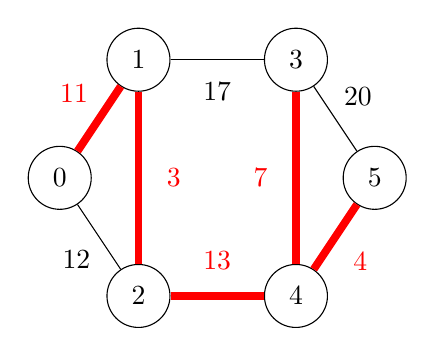
\begin{tikzpicture}[scale=1, every node/.style={circle, draw, minimum size=8mm}]

        % Nós 
        \node (0) at (0,1.5) {0};
        \node (1) at (1,3) {1};
        \node (2) at (1,0) {2};
        \node (3) at (3,3) {3};
        \node (4) at (3,0) {4};
        \node (5) at (4,1.5) {5};

        % Arestas normais
        \draw (0) -- node[below left, draw=none, midway] {12} (2);
        \draw (1) -- node[below, draw=none, midway] {17} (3);
        \draw (3) -- node[above right, draw=none, midway] {20} (5);

        % Arestas da AGM 
        \draw[red, line width=1.0mm] (0) -- node[above left, draw=none, midway] {11} (1);
        \draw[red, line width=1.0mm] (1) -- node[right, draw=none, midway] {3} (2);
        \draw[red, line width=1.0mm] (2) -- node[above, draw=none, midway] {13} (4); 
        \draw[red, line width=1.0mm] (4) -- node[below right, draw=none, midway] {4} (5);
        \draw[red, line width=1.0mm] (4) -- node[left, draw=none, midway] {7} (3);

    \end{tikzpicture}

    \caption{Exemplo de grafo ponderado com nós 0,1,2,3,4,5 e sua Árvore Geradora Mínima.}%
    \label{fig:exemplo_grafo}
\end{figure}

Neste exemplo, a AGM seleciona as arestas com menores pesos que permitem conectar todos os vértices sem ciclos, minimizando o custo total:

\[
    E_{\text{AGM}} = \{(0,1,11), (1,2,3), (2,4,13), (4,3,7), (4,5,4)\}, \quad C_{\text{total}} = 38
\]



% 5. MODELAGEM DO PROBLEMA
\section{Modelagem do Problema}%
\label{sec:modelagem}

A Árvore Geradora Mínima (AGM) pode ser formulada por um \textit{single-commodity flow model}, no qual o fluxo enviado pelo nó raiz garante conectividade e impede ciclos sem usar restrições de corte.

Seja $G = (V,E)$ um grafo não direcionado, onde $V = \{0,1,\ldots,n-1\}$ e o vértice $0$ atua como raiz.

\subsection{Variáveis de Decisão}

\begin{itemize}
    \item $x_{uv} \in \{0,1\}$: indica se a aresta $(u,v)$ faz parte da AGM.\@
    \item $f_{uv} \ge 0$: fluxo enviado de $u$ para $v$, permitido apenas em arestas ativas.
\end{itemize}

\subsection{Função Objetivo}

\begin{equation}
    \min \sum_{(u,v)\in E} w_{uv}\, x_{uv}
\end{equation}

\subsection{Restrições}

\paragraph{(a) Conservação de Fluxo}

Na raiz:

\begin{equation}
    \sum_{v \in V} f_{0v} - \sum_{v \in V} f_{v0} = n-1
\end{equation}

Nos demais vértices:

\begin{equation}
    \sum_{u \in V} f_{u v} - \sum_{w \in V} f_{v w} = 1,
    \quad \forall v \in V \setminus \{0\}
\end{equation}

\paragraph{(b) Capacidades (ligação fluxo–aresta)}

\begin{equation}
    f_{uv} \le (n-1)x_{uv}, \quad \forall (u,v)\in E
\end{equation}

\begin{equation}
    f_{vu} \le (n-1)x_{uv}, \quad \forall (u,v)\in E
\end{equation}

\paragraph{(c) Cardinalidade das Arestas}

\begin{equation}
    \sum_{(u,v)\in E} x_{uv} = n-1
\end{equation}

\paragraph{(d) Domínio das Variáveis}

\begin{align}
    x_{uv} &\in \{0,1\}, && \forall (u,v)\in E \\
    f_{uv} &\ge 0,       && \forall (u,v)\in E
\end{align}

\noindent
Essa formulação garante que a solução seja uma árvore conexa, acíclica e de custo mínimo.


% 6. DADOS DO PROBLEMA
\section{Dados do Problema}%
\label{sec:dados_problema}

Os dados utilizados neste trabalho referem-se a um grafo não direcionado $G = (V, E)$, no qual $V$ representa o conjunto de vértices e $E$ o conjunto de arestas com pesos associados. Essas informações estão armazenadas no arquivo \texttt{arvore\_geradora\_minima.txt}, utilizado como entrada para o modelo.

\subsection*{Estrutura do Arquivo}%
\label{sec:estrutura_arquivo}

O arquivo apresenta uma linha por aresta, contendo três valores: os vértices conectados e o peso da aresta. Esse formato facilita a leitura por programas de otimização e permite construir o grafo diretamente a partir do arquivo.

\begin{itemize}
    \item \textbf{Vértices:}  
    Os vértices são identificados por números inteiros sequenciais. No conjunto utilizado, temos:
    \[
        V = \{0,1,2,\ldots,49\}
    \]
    Essa numeração simplifica o tratamento computacional e a indexação no modelo.

    \item \textbf{Arestas e pesos:}  
    Cada linha do arquivo segue o padrão:
    \[
        (u,v,w_{uv}),
    \]
    onde $u$ e $v$ são os vértices conectados e $w_{uv}$ é o peso da aresta. Exemplo extraído:
    \[
        E = \{(0,1,44), (1,2,18), (2,3,5), \ldots, (28,46,35)\}.
    \]
    Esses pesos compõem os coeficientes da função objetivo do modelo.

    \item \textbf{Formato:}  
    A organização em três colunas torna o arquivo compacto e facilmente processável, permitindo sua conversão imediata para estruturas de dados adequadas à representação do grafo.

\end{itemize}

\subsection*{Uso dos Dados no Modelo}%
\label{sec:dados_modelo}

As informações do arquivo permitem:

\begin{itemize}
    \item identificar todas as arestas disponíveis no grafo;
    \item associar pesos $w_{uv}$ às variáveis $x_{uv}$;
    \item definir o conjunto $E$ utilizado nas restrições de fluxo e cardinalidade.
\end{itemize}

Dessa forma, o arquivo fornece todos os elementos necessários para construir o grafo e aplicar o modelo matemático que determina a árvore geradora mínima.


% 7. RESULTADOS
\section{Resultados}%
\label{sec:resultados}

A aplicação do modelo de Programação Linear Inteira permitiu determinar a solução ótima do problema da Árvore Geradora Mínima (AGM). As arestas selecionadas minimizam o custo total, respeitando as restrições de conectividade e evitando ciclos, conforme definido no modelo matemático.

\subsection{Arestas Selecionadas}%
\label{sec:arestas_selecionadas}

Com base nas variáveis de decisão \(x_{uv}\) do modelo, as arestas incluídas na AGM são aquelas para as quais \(x_{uv} = 1\):

\[
\begin{aligned}
    E_{\text{AGM}} = \{ & (2,3), (5,6), (8,9), (9,10), (11,12), (15,16), (24,25), \\
    & (28,29), (31,32), (35,36), (36,37), (39,40), (48,49), (24,42), (15,45), \\
    & (20,23), (6,17), (26,32), (24,49), (33,36), (24,43), (17,31), (12,29), \\
    & (8,19), (35,49), (13,28), (31,43), (19,40), (16,42), (26,34), (38,40), \\
    & (22,42), (39,41), (0,6), (1,30), (18,26), (7,46), (28,44), (4,19), (7,45), \\
    & (21,41), (25,27), (39,47), (8,20), (15,19), (28,39), (1,48), (2,18), (14,34) \}
\end{aligned}
\]

Estas arestas conectam todos os vértices do grafo, formando um grafo conexo e acíclico, atendendo às restrições do modelo.

\subsection{Custo Total}%
\label{sec:custo_total}

O custo total da AGM, calculado somando os pesos \(w_{uv}\) das arestas selecionadas, é:

\[
    C_{\text{total}} = 433
\]

Esse valor representa o menor custo possível para interligar todos os vértices, confirmando que a solução encontrada é ótima de acordo com a função objetivo:

\[
    \min \sum_{(u,v)\in E} w_{uv} \, x_{uv}.
\]

\subsection{Relação com o Modelo Matemático}%
\label{sec:relacao_modelo}

As variáveis de decisão do modelo são \(x_{uv} \in \{0,1\}\), indicando se a aresta \((u,v)\) foi incluída na AGM.\@ A função objetivo consiste na minimização do custo total, conforme apresentado acima.

As restrições do modelo foram atendidas de acordo com a solução ótima encontrada:

\textbf{1. Quantidade de arestas:} A soma das variáveis de decisão é igual a \(n-1\), garantindo que a AGM possua exatamente o número correto de arestas.

\textbf{2. Evitar ciclos:} As arestas selecionadas formam um grafo acíclico, assegurando que não existam ciclos na árvore.

\textbf{3. Domínio das variáveis:} Cada variável de decisão satisfaz \(x_{uv} \in \{0,1\}\), garantindo que a solução seja discreta e represente corretamente a presença ou ausência de cada aresta na AGM.\@

Dessa forma, os resultados demonstram que o modelo matemático implementado gerou uma solução ótima, com todas as restrições respeitadas e custo total mínimo.


% 8. CONCLUSÕES
\section{Conclusões}%
\label{sec:conclusoes}

O estudo desenvolvido ao longo deste trabalho permitiu explorar de maneira abrangente o problema da Árvore Geradora Mínima (AGM), desde seus fundamentos teóricos até a formulação matemática e obtenção de resultados ótimos por meio de Programação Linear Inteira. A AGM constitui um dos problemas fundamentais em teoria dos grafos e otimização combinatória, e sua resolução exata por métodos matemáticos reforça não apenas sua relevância prática, mas também o valor das técnicas de modelagem aplicadas.

Inicialmente, discutiu-se a estrutura do problema e seus requisitos essenciais: conectividade entre todos os vértices, ausência de ciclos e minimização do custo total associado às arestas selecionadas. Em seguida, abordou-se a formulação matemática clássica, destacando suas limitações, especialmente no que diz respeito às restrições de corte, que possuem caráter exponencial e podem tornar o modelo computacionalmente inviável para instâncias maiores.

A partir disso, introduziu-se a formulação baseada em fluxo (\textit{single-commodity flow}), que representa uma alternativa eficiente e elegante para modelar a conectividade do grafo. Essa abordagem evita explicitamente a necessidade de restrições de corte ao empregar um artifício de conservação de fluxo que garante, de maneira natural, que todos os vértices sejam alcançáveis a partir de um nó raiz. A utilização simultânea de variáveis binárias \(x_{uv}\) e variáveis de fluxo \(f_{uv}\) permitiu expressar de maneira rigorosa a dependência entre a seleção de uma aresta e a possibilidade de transporte de fluxo através dela. As restrições de capacidade desempenharam papel crucial nesse vínculo, assegurando que nenhum fluxo circulasse por arestas inativas.

Os resultados computacionais reforçaram a coerência e a funcionalidade da modelagem. As arestas selecionadas compõem um conjunto de exatamente \(n - 1\) elementos, formando uma estrutura conexa e acíclica, conforme exigido para uma AGM.\@ O custo total obtido, \(C_{\text{total}} = 433\), confirma que o modelo identificou a solução ótima, consistente com a função objetivo e com todas as restrições impostas. A análise do conjunto de arestas demonstra, ainda, que o fluxo se distribuiu de maneira válida pela estrutura final, validando tanto a conservação quanto a utilização do fluxo como mecanismo de conectividade.

Em síntese, o trabalho realizado demonstra que a formulação por fluxo constitui não apenas uma forma exata e eficiente de resolver a AGM, mas também um arcabouço flexível, capaz de acomodar extensões e variações do problema original. A combinação entre rigor matemático, clareza estrutural e eficiência computacional torna essa abordagem particularmente adequada tanto para ambientes acadêmicos quanto para aplicações reais em áreas como redes de computadores, sistemas logísticos, planejamento de infraestrutura e engenharia de produção. Dessa forma, este estudo evidencia o potencial e a relevância da Programação Linear Inteira como ferramenta poderosa na solução de problemas de otimização sobre grafos.


\end{document}